\clearpage
\subsection{Machine Code} % (fold)
\label{sub:machine_code}

\emph{What instructions do Computers understand?}

Computers do not really \emph{understand} anything, computers are \textbf{unintelligent}. They are a machine that respond in a set way to a given number of instructions. The instructions that a computer uses is called its {\em instruction set} and contain instructions to perform basic mathematic operations, loading and storing data in memory, comparing numeric values, and moving to the new instruction elsewhere in the program. These very simple actions are performed very quickly, and can be use to create everything you have ever seen a computer do.

The computers instructions can be seen as binary numbers, numbers made from 0's and 1's. These values are like switches that are either off (0) or on (1). Setting these \emph{switches} to different sequences will cause the computer to perform different actions. For example, the \emph{switch} combination \texttt{0000 0011}, may cause the computer to add two numbers together. Any time you want the computer to perform this task you set the switches to that combination. These binary instructions are called \textbf{machine code}.

\begin{figure}[h]
   \centering
   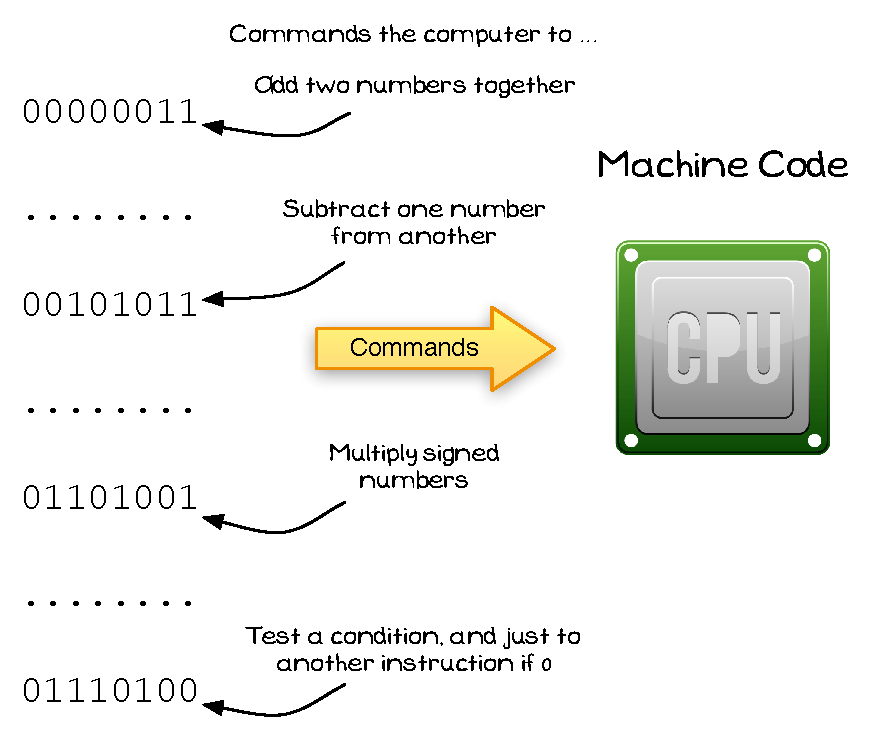
\includegraphics[width=0.8\textwidth]{./topics/programs-and-compilers/diagrams/MachineCode} 
   \caption{The computer responds to machine code instructions}
   \label{fig:machine-code}
\end{figure}

\mynote{
\begin{itemize}
  \item The \textbf{CPU}, Central Processing Unit, is the workhorse of the computer. It executes the program's instructions.
  \item The instructions a CPU uses is called its \textbf{Instruction Set}, and different CPUs have different instruction sets.
  \item Some common instruction sets: ARM (used in iPhones and iPads), x86-64 (used in desktops), and PowerPC (used in the XBox360 and Playstation 3). 
\end{itemize}
}

\clearpage

\subsubsection{Programming in Machine Code} % (fold)
\label{ssub:programming_in_machine_code}

Listing \ref{lst:machine code} shows a chunk of the machine code for a small program. These 1s and 0s are the codes used to instruct the computer when this program is executed. Programs can be written directly in machine code, but this is a time consuming task. This is further complicated by the fact that machine code is unique to each kind of CPU. This means that programming at this level is entirely dependent on the kind of processor that you are targeting.

\begin{lstlisting}[caption={128 bits from the 106,752 bits of Machine Code from a small program.},label={lst:machine code}]
...
0110 0111 0111 0010 0000 0000 0110 0011 0100 1110 0101 1111 0100 0001 0101 1000
0110 0111 0111 0010 0000 0000 0111 0110 0101 1111 0101 1111 0110 1001 0101 1111
...
\end{lstlisting}

No one wants to have to work at this level of details, and fortunately you do not need to. Software developers have created tools to help them create programs without having to think about these low level details. These tools make it possible to work at a \textbf{higher level of abstraction}. They take the code you write, and do the hard work of converting that to the machine code of the computer you want to run it on.

\mynote{
\begin{itemize}
  \item You can look at the machine code of any program on your computer. You just need the right tools.
  \item If you open the program's executable file in a text editor it will look very strange, and not at all like a large list of binary values. This is because the text editor displays one character for every byte (or two bytes depending on the file) from the file.
  \item A \textbf{Hex Editor} is a program that is useful for examining binary data. It shows you one character for every four bits in the file.
\end{itemize}
}

\begin{table}[h]
  \ttfamily
  \centering
\begin{tabular}{|c|c||c|c||c|c||c|c|}
  \hline
  Binary & Hex & Binary & Hex & Binary & Hex & Binary & Hex  \\
  \hline
  0000 & \textbf{0} & 0001  & \textbf{1}  & 0010  &  \textbf{2} & 0011 & \textbf{3} \\
  0100 & \textbf{4} & 0101 & \textbf{5} & 0110 & \textbf{6} & 0111 & \textbf{7} \\
  1000 & \textbf{8} & 1001 & \textbf{9} & 1010 & \textbf{A} & 1011 & \textbf{B} \\
  1100 & \textbf{C} & 1101 & \textbf{D} & 1110 & \textbf{E} & 1111 & \textbf{F} \\
  \hline
\end{tabular}
  \caption{Binary to Hexadecimal}
\end{table}

\begin{figure}[h]
   \centering
   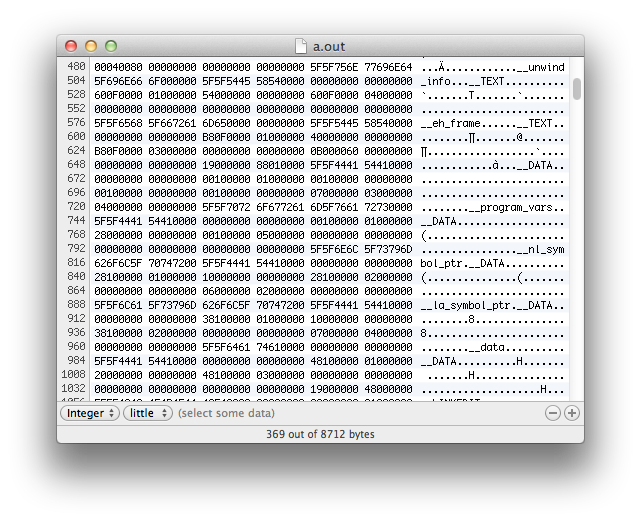
\includegraphics[width=0.55\textwidth]{./topics/programs-and-compilers/images/HexEditor} 
   \caption{A HexEditor allows you to view the machine code of any program}
   \label{fig:hex-editor}
\end{figure}


% subsubsection programming_in_machine_code (end)

% subsection machine_code (end)